\lecture{Thu. 9/6/12}

Today Bill Minicozzi (2-347) is filling in for Toby Colding.

We will follow the textbook \ul{Riemannian Geometry} by Do Carmo. You have to spend a lot of time on basics about manifolds, tensors, etc. and prerequisites like differential topology before you get to the interesting topics in geometry. Do Carmo gets to the interesting topics much faster than other books.

Today we give a quick overview of Riemannian geometry, and then introduce the basic definitions (manifolds, tangent spaces, etc.) that we'll need throughout the course. You will see how these definitions generalize concepts you are already familiar with from calculus. %such as the directional derivative.

\subsection{What is Riemannian geometry?}

%Riemannian geometry
On Euclidean space we can do calculus; we can measure distances, angles, volumes, etc.

However, we want to do all that geometry on more general spaces, called \textbf{Riemannian manifolds}.

First, we'll have to rigorously define what those spaces are. What is a manifold? We need to generalize the basic notions of calculus in the manifold setting: what is a derivative? A derivative is basically a linear approximation, because the tangent line is the best linear approximation. We'll define the notion of a \textbf{tangent space} for a manifold.
%painful but allows more interesting.

Once we have a manifold, we can define have functions, curves and (sub)surfaces on the manifolds, and objects called \textbf{tensors}. %A function is well-defined on each point (to $\R$). 
The idea of tensors generalizes the idea of vector fields, which are 1-tensors. We can differentiate tensors; for instance, the covariant derivative of two-tensor is three-tensor.

%10 minutes late

Next, we'll see that a \textbf{Riemannian metric} allows us to calculuate distance and angles. A \textbf{geodesic} is the shortest path connecting two points, or more generally, paths that are {\it locally} shortest. For instance, the equator of a sphere is a geodesic: any connected part of the diameter that doesn't include antipodal points gives the shortest path between two points. We can view our spaces as metric spaces and do some geometry. We have \emph{comparison theorems}, where we use the geometry of the space to get information about the metric. For instance, in the Bonnie-Meyer theorem, we use the curvature of a space to learn about its metric. 

Later in the course, we will cover topic such as Cartan-Hadamard manifolds, harmonic maps, and minimal surfaces.

\subsection{Manifolds}

We want to do calculus on more general spaces, called manifolds. In particular, we care about (smooth) differential manifolds. Before we give a formal definition, we first develop some intuition through examples.

\subsubsection{Examples}

The following are all manifolds.
\begin{itemize}
\item
$\R^n$: $n$-dimensional Euclidean space 
\[\R^n:=\set{(x_1,\ldots,x_n)}{x_i\in \R}.\]
\item
$S^n$: the unit $n$-sphere 
\[S^n:=\set{x\in \R^{n+1}}{|x|=1}.\]
Here the Euclidean norm is defined by $|x|^2:=\sum_{i=1}^n x_i^2$. Note this is an example of a ``submanifold" of $\R^{n+1}$. %Curves and surfaces book
%submanifolds of Euclid space. Curve of submanifold, in Euclidean space
%notion of distances.
 %But it's better not  assume
\end{itemize}
Note that Euclidean geometry descends to geometry on any submanifold. A theorem of Nash says any abstract manifold can be embedded (at least locally) in Euclidean space. This means it is sufficient to learn about geometry of submanifolds of Euclidean space. %Just restrict what we already know how to do in $\R^n$.  For instance, we only have to define harmonic space in Euclidean space, rather than define it for an abstract manifold.

However, just as linear algebra is often simpler with ``linear transformations" than with matrices, we will see that geometry is often simpler when we think of manifolds in the abstract.

Here are some more examples.
\begin{itemize}
\item
$T^n$: $n$-torus $\R^n/\Z^n$. This means that we are modding out $\R^n$ by the equivalence relation $\sim$ where $x\sim (x+z)$ for every tuple $z=(z_1,\ldots, z_n)$ with $z_i\in \Z$. Note any small piece of $T^n$ looks like $\R^n$ because don't see the wraparound. 

This local property means we can calculate derivatives of a function defined on $T^n$ the same way we calculate derivatives of a function on $\R^n$.
\item
$\RP^n$: real projective $n$-space, the space of lines through 0 in $\R^{n+1}$. Note $\RP^n$ is closely related to the $S^n$, as follows. Each line through origin cuts sphere in 2 points, so we can think of $\RP^n$ as $S^n$ modded out by the antipodal map $p\mapsto -p$.
\end{itemize}
These are all differential manifolds, %because they all have differential geometry. 
but we don't get a {\it geometry} on them until we get a Riemannian metric (something we'll develop later in the course).

We also need a notion of a tangent vector. We'll give a formal definition of a manifold, then go back to talk about tangent spaces on manifolds.

%Submanifold induces geometry. Does geometry determine embedding? Uniqueness or rigidity question. Some cases knowing. If convex, should essential determine geometry up to rotation. Submanifold of E space. Translate whole thing, haven't changed. Is rigid transformation only thing mod out by.

\subsubsection{Formal definition}

\begin{df}
A (smooth) $n$-dimensional \textbf{manifold} $M$ is...
\begin{enumerate}
\item
a set, denoted $M$, equipped with
\item 
a family of open sets $U_{\al}\subeq \R^n$ and injective maps $x_{\al}:U_{\al}\hra M$ (together called a \textbf{chart}) such that
\begin{itemize}
\item
(The open sets cover the manifold) $\bigcup_{\al} x_{\al}(U_{\al})=M$. 
\item
(Overlap properties) Set $W_{\al\be}:=x_{\al}(U_{\al})\cap x_{\be}(U_{\be})$ for each $\al$ and $\be$. Suppose $W_{\al\be}\ne \phi$.
%every point can find ball contained in
Then 
\begin{enumerate}
\item
$x_{\al}^{-1}(W_{\al\be})$ is open,
\item
$x_{\be}^{-1}\circ x_{\al}$ is $C^{\iy}$, i.e. infinitely differentiable %(for smooth manifold)
\item
(*) This family is maximal with respect to A and B.
\end{enumerate}
 %(Real analytic, complex---$\C^n$ holomorphic) PL manifolds piecewise linear. Lots of flexibility in notion. Something categorical going on. 
\end{itemize}
\end{enumerate}
%Maximal means with respect to set inclusion.
\end{df}

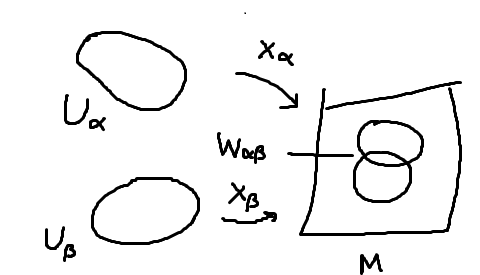
\includegraphics{1-1}

Let's analyze this definition. 
The open sets $U_{\al}$ tell us that locally, each point is  parameterized by an open set in Euclidean space. %Essential notion of manifolds. 
We saw this in each of the examples. (For $S^n$, you can ``flatten" any local part of the sphere.) 
Note that $M$ inherits a topology by deeming that each $x_{\al}(U_{\al})$ be a homeomorphism onto an open set of $M$.

The technical overlap properties force the $x_{\al}$ to be nice maps. (b) is why we call the manifold ``smooth." We can loosen, tighten, or change the condition, for instance,
\begin{itemize}
\item A real analytic manifold is where $x_{\be}^{-1}\circ x_{\al}$ are all real analytic.
\item A complex manifold is one where we replace $\R$ with $\C$ and $C^n$ by holomorphic.
\item A PL manifold is where $x_{\be}^{-1}\circ x_{\al}$ are all piecewise linear.
\end{itemize}

Without condition (c), we would have a lot of manifolds. Suppose we have $(M,\{x_{\al}\},\{U_{\al})$ satisfying all the conditions except (c). For each $U_{\al}$, we can take a subset $V\subeq U_{\al}$ and restrict $x_{\al}$ to $V$. This is still a good parameterization. Adding $V$ and $x_{\al}|_V$, we get a new manifold. 
%Without C they would be different manifolds. 

Thus (c) gives uniqueness: two manifolds that should be the same {\it are} the same.

An alternative approach is as follows: call something satisfying just (a) and (b) quasi-manifolds. Define an equivalence relation: two manifolds are the same if you can refine the two families of mappings $\{(U_{\al},x_{\al})\}$ to be the same family. Modding out quasi-manifolds by this equivalence relation gives a manifold.

Note $n$ has to be constant: A sphere with two 1-dimensional antlers is not a manifold.

\subsubsection{Reconciling definition with example}

Let's show that $\RP^n$ is a manifold. Define \textbf{homogeneous coordinates} as follows: 
Consider $\set{(x_1,\ldots, x_{n+1})\in \R^{n+1}}{\text{at least one }x_i\ne 0}$, and mod out by the equivalence relation
%$[x_1,\ldots, x_{n+1}]$ with at least one $x_i\ne 0$ is the equivalence class of $(x_1,\ldots, x_{n+1})$ with equivalence relation
\[
(x_1,\ldots, x_{n+1})\sim \la (x_1,\ldots, x_{n+1})
\]
where $\la\in \R\bs \{0\}$. Let the $[x_1,\ldots, x_{n+1}]$ denote the equivalence class of $(x_1,\ldots, x_{n+1})$; it is called homogeneous coordinates.\\

\noindent \underline{Defining the open sets and maps:}\\


Define sets $V_i=\set{[x_1,\ldots, x_{n+1}]}{x_i\ne 0}$. It's clear that $\bigcup V_i=\RP^n$.  Because we need to get $n+1$ coordinates out of $n$ coordinates, we define maps $x_i:\R^n\to V_i$ by
\[
x_i(y_1,\ldots, y_n)=[y_1,\ldots, \underbrace{1}_i,\ldots, y_n].
\]

For instance, for $\RP^3$, we have
\bal
x_1(y_1,y_2)&=[1,y_1,y_2]\\
x_2(y_1,y_2)&=[y_1,1,y_2]\\
x_3(y_1,y_2)&=[y_1,y_2,1]
\end{align*}
Note these maps are all bijective. They are onto because any element of $[x_1,\ldots, x_n]\in V_i$ has $x_i\ne 0$, and $[x_1,\ldots, x_n]=\ba{\fc{x_1}{x_i},\ldots ,\fc{x_i}{x_i}=1,\ldots, \fc{x_n}{x_i}}$.\\

%We see that each $x_i$ is bijective to $V_i$. 
\noindent\underline{Verifying overlap properties:}
\begin{enumerate}
\item[(a)]
%The set 
We have
\[W_{12}=x_1(\R^2)\cap x_2(\R^2)=V_1\cap V_2=\set{[z_1,z_2,z_3]}{z_1z_2\ne 0}.\] 
%is open because $z_1z_2$ is a continuous function, and ``$\ne0$" is an open condition.
%\item[(b)]
Consider $x_1^{-1}(W_{12})$. We have $[z_1,z_2,z_3]\sim \ba{1,\fc{z_2}{z_1},\fc{z_3}{z_1}}$, so
\[
x_1^{-1}W_{12}=\set{(y_1,y_2)}{y_1\ne 0}.
\]
which is open.
%We just verified the first part of B. 
\item[(b)]
Now consider $x_2^{-1}\circ x_1:W_{12}\to W_{21}$. We have for $y_1\ne 0$ that
\[
(y_1,y_2)\xra{x_1}[1,y_1,y_2]=\ba{\rc{y_1},1,\fc{y_2}{y_1}}\xra{x_2^{-1}} \pa{\rc{y_1},\fc{y_2}{y_1}}.
\]
This is rational, so smooth.
\item[(c)] To satisfy condition (c), we take a maximal family of $(V_{\al},x_{\al})$ satisfying (a) and (b) and containing all the $(V_i,x_i)$. (I.e. take all intersections among all the $(V_i,x_i)$ and add them in; now take all subsects, not take intersections again, {\it ad infinitum}.)
\end{enumerate}
%Now throw in all open subsets of the $U_{\al}$ and intersections, restrictions of those, until we get something maximal.

Because the calculations are straightforward, this is the first and last time we're going to check something is a manifold.

\subsubsection{Maps between manifolds}
\begin{df}
Let $M$ and $N$ be smooth manifolds.
We say that $\ph:M\to N$ is smooth at $p\in M$ if $x_N^{-1}\circ \ph\circ x_M$ is smooth at $x_M^{-1}(p)$.

Here, $x_M$ is any $x_{\al}$ such that $p\in x_{\al}(U_{\al})$, and $x_N$ is any $x_{\be}$ such that $\ph(p)\in x_{\be}(U_{\be})$.
\end{df}

\begin{center}
\includegraphics{1-2}
\end{center}

Note the choice of $x_M=x_{\al}$ and $x_N=x_{\be}$ doesn't matter, because the transition condition will give that it is true for any choice.

Some particularly important smooth maps are those with domain or target inside $\R$:
\begin{itemize}
\item
Smooth functions on $M$, i.e. smooth maps $M\to \R$. This set is denoted by $\cal D$.
\item
Curves, maps from an interval $I\subeq \R\to M$.
\end{itemize}

\subsection{Tangent vectors}

%Tangent vector obvious for submanifold, descend.

%Some books bring in notion of tensor. Once we go to charts. When change coordinates, change in certain way. (Computational notion of derivative). Do Carmo better approach: invariant under choice of charts. Can be express in coordinates, forced a certain way to change. (Other: something that changes in coordinates that way) \fixme{Explain better.}
There are two approaches to defining the derivative of a function on a manifold. 
\begin{itemize}
\item
The computational approach is to give it in terms of coordinates. We have to define how it transforms when we change coordinates.
\item
We can define it in a more abstract way, invariant under choice of charts. This is Do Carmo's approach and the approach we'll take. This automatically forces what the derivative has to be when we \emph{do} express it in coordinates.
\end{itemize}

We'll first look at derivatives/tangent vectors in $\R^n$, and then generalize to manifolds.
\subsubsection{Tangent vectors in $\R^n$}
\begin{df}
Let $\al:(-\ep,\ep)\to \R^n$ and $f:\R^n\to \R$ be smooth, so that $f\circ \al$ is a smooth function $(-\ep,\ep)\to \R$.
%Calculus gives us $(f\circ \al)'(0)$. 
Define the \textbf{directional derivative} or \textbf{tangent vector} in the direction of $\al$ of $f$ to be 
%The \textbf{directional derivative}
\[
(f\circ \al)'(0)=\sum_{i=1}^n \pd{f}{x_i} (\al(0))\al_i'(0)=\an{\nabla f,\al'(0)}.
\]
(The equality is by the chain rule.)
Thus, we can think of the tangent vector as a function sending $\al$ to the linear map $f\mapsto \an{\nabla f,\al'(0)}$.
\end{df}
Note the derivative depends only on $\al'(0)$. It didn't matter what the curve was; we could have covered all possibilities with curves that are straight lines, $\al(t)=p+tq$.

\begin{df}
A \textbf{derivation} $D$ of an $\R$-algebra $A$ is a $\R$-linear function from $A$ to $\R$ that satisfies the Leibniz rule \[D(fg)=(Df)g+f(Dg),\qquad f,g\in A.\]
Denote the space of derivations by $\Der(A)$.
\end{df}
%\begin{thm}\llabel{18965-1-1}
\begin{pr}
Let $C^{\iy}(x_1,\ldots, x_n)$ be the set of $C^{\iy}$ functions on $x_1,\ldots, x_n$.
The map $v\mapsto (f\mapsto \an{\nabla f,v})$ is a vector space isomorphism from $\R^n$ to $\Der(C^{\iy}(x_1,\ldots, x_n))$.
\end{pr}
(Proof of surjectivity is omitted.) Think of $v$ as $\al'(0)$, so the map is
\[
f\mapsto \an{\nabla f,\al'(0)}.
\]

Now why did we define the directional derivative in terms of $\al$ instead of $v=\al'(0)$? Because we want something that {\it doesn't depend on coordinates}. Associated to $\al$ we get a {\it linear map} $f\mapsto \an{\nabla f,\al'(0)}$ that we can define without coordinates. This is why we define the tangent vector as a linear map on a space of functions.\\

\cpbox{We define the tangent vector to be a linear map on a space of functions, so that it does not depend on coordinates.}
\vskip0.15in
This will be important in the general manifold setting.

%\begin{proof}[Proof of Theorem~\ref{18965-1-1}]
%We just have to show all the derivations are given by $f\mapsto \an{\nabla f,v}$ for some $v$.
%\end{proof}
%
%%identify
%We have an equivalence $\al'(0)\in \R^n$ we get a linear operator (derivation: linear and satisfy Leibniz rule) from smooth functions to $\R$ sending
%%lots of linear maps. map to second derivative, etc. Need restrictions.
%\[
%
%\]
%We want a coordinate-free description of tangent vector: as a linear map.

%\fixme{(Chain rule statement gives one-one correspondence between vectors in $\R^n$ and directional derivatives (tangent space to itself))}

%This is just on $\R^n$.

\subsubsection{Tangent vectors in general}
Our viewpoint naturally generalizes to manifolds.
\begin{df}
Let $\al:(-\ep,\ep)\to M$ be a smooth curve. Then define the tangent vector as the linear map $\al'(0):\cal D\to \R$ given by
\[
\al'(0)f=(f\circ \al)'(0)
\]
The \textbf{tangent space} to $M$ at $p$ is
\[
T_pM=\{\text{All tangent vectors to curves through }p\}
\]
\end{df}
Note that $T_p\cong \R^n$. We will explain why.

To actually perform computations involving tangent vectors, we need to work on the actual charts, so the maps $(-\ep,\ep)\xra{\al} M \xra{f} \R$ are unsatisfactory. So given a point $p$, let
%mat vs. lin trf
$x:U\to M$ be a parameterization around $p$. Then we can work on the chart $U$, because we have the following commutative diagram (for small enough $\ep$)
\beq{18965-1-cd}
\xymatrix{
(-\ep,\ep)\ar[r]^{\al}\ar[rd]_{x^{-1}\circ \al} & M \ar[r]^f & \R\\
& U \ar[ru]_{f\circ x} \ar[u]_x& 
}
\eeq 
Note $(-\ep,\ep)\xra{x^{-1}\circ \al}U\xra{f\circ x}\R$ are maps staying in $\R$, so we can do multivariable calculus with them.

\begin{center}
\includegraphics{1-3}
\end{center}

Write
\bal
x^{-1}\circ \al(t)&=(\al_1(t),\ldots, \al_n(t))\\
f\circ x(x_1,\ldots, x_n)&=f(x_1,\ldots, x_n)\text{ as shorthand}\\
(f\circ \al)(t)&=(f\circ x)\circ (x^{-1}\circ \al)(t).
\end{align*}

The chain rule gives
\[
\sum_{i=1}^n \pd{f}{x_i} \al_i'(0).
\]
(By abuse of notation $\pd{f}{x_i}=\pd{f\circ x}{x_i}$ and $\al_i'(0)$ is the $i$th component of $(x^{-1}\circ \al)'(0)$.) Think of this as the directional derivative ``in coordinates," just like we can express a linear transformation as a matrix once we have coordinates.

Now if we had a different $(V,x')\ne (U,x)$ with $p\in x'(V)$, we can add $V$ to our commutative diagram~\eqref{18965-1-cd}
We can then compute the directional derivative in the coordinates of the chart $V$ instead of $U$, and we can see how the derivative changes from $U$ to $V$ using the chain rule on $y^{-1}\circ x$. %Write the whole thing out with coordinates in between. Extra terms. Derive way vector expression changes when chg coord

Thus we see that the directional derivative is an invariant notion---we don't need coordinates to define it, but once we do have coordinates, we can calculate it in terms of coordinates, and we know exactly how this expression changes when we change coordinates.

One thing to note is that if the $\al'(0)$ are all 0, then no matter \emph{what} coordinates we choose, all the $\al_i'$ are still 0. But if $\al'(0)$ is nonzero, then we can mix things up any way we like.

Remarks:
\begin{enumerate}
\item
$\al'(0)$ depends only on $\al'(0)$ in a coordinate system.
\item
$T_p(M)$ is a $n$-dimensional vector space with a natural basis
\[
\pd{}{x_i}:=\text{tangent vector to curve where we only vary }x_i.
\]
(More precisely, we are considering the curve $\al(t)=x(x^{-1}(p)+tx_i)$.) We have $\al_i'(0)=\de_{ij}$.
\end{enumerate}•
%n of them, lin indpt, bijective.
%def'd w/o reference to coord sys. When doing problems, introduce coord system.

\subsection{Differentials}
\begin{df}
A smooth map $\ph:M\to N$ induces linear maps
\[
d\ph_p:T_pM\to T_{\ph(p)}N
\]
%move all curves over
by taking the curve $\al$ to curve $\ph\circ \al$:
\[
d\ph_p(\al'(0)):= (\ph\circ \al)'(0).
\]
The map $d\ph_p$ is called the \textbf{differential} of $\ph$ at $p$.
\end{df}
%\fixme{
%Exercise: doesn 
Again this does not depend on the choice of $\al$, only on $\al'(0)$.\\
%}

\cpbox{Any smooth map $\ph$ gives rise to a differential map on the tangent spaces.}
\vskip0.15in
Once we have the differential, we can talk about immersions and embeddings. 
\begin{df}
We say that 
$\ph:M\to N$ is a diffeomorphism if it is
\begin{enumerate}
\item
smooth
\item
bijective, and
\item $\ph^{-1}$ is smooth.
\end{enumerate}
\end{df}
\begin{df}
We say that $\ph:M\to N$ is a \textbf{local diffeomorphism} at $p\in M$ if there exists an open set $U$ containing $p$ such that $\ph_i:U\to \ph(U)$ is a diffeomorphism
\end{df}
\begin{df}
$\ph:M\to N$ is an \textbf{immersion} if $d\ph_p$ is \emph{injective} at each $p$.
\end{df}
We have the following theorem
\begin{thm}[Inverse function theorem for manifolds]
If $d\ph_p$ is bijective, then $\ph$ is local diffeomorphism to $p$.
\end{thm}
This tells us that if the linearization of $\ph$, i.e. $d\ph_p$, is a bijection at $p$, then  $\ph$ is actually a diffeomorphism at $p$.
\begin{proof}
Appeal to Euclidean Inverse Function Theorem (see Analysis on Manifolds, by Munkres) and compose with charts at either end.
\end{proof}
%Diff'l invertible at point.